\chapter{MODELING}
\label{chapter:modeling}

\par
The modeling phase included getting familiar with concepts of \acrshort{bsc}, creating the behavioral models for most of its functional parts, verifying its correctness and  defining the layered structure or models.

\section{Brainloop Secure Client app for iOS platform} 

\par
In order to deeply understand the concept behind \acrshort{bsc} we need to first have a good understanding of the Brainloop Secure Dataroom Service (\acrshort{bdrs}). 

\par
\acrshort{bdrs} \cite{BDRS_Description} is a secure service for data governance, allowing customer businesses reliable and extremely secure data and communication management within the company as well as with outside parties such as partners, consultants, government agencies and clients. Highest level of security is achieved with double authentication with time-limited PINs, 256-bit encryption of storage as well as data transfer, consistent separation of application and system administration and other state-of-the-art security features available. Document management is supported with multiple features such as structured filing, editing and distribution of documents, document collections that combine, sort and structure several documents with separate version management and different access rights, automatic generation of protected PDF files from PDF, Office documents and picture files for write-protected access with layout checks, where required with additional security options, such as print prevention or content exports, version management and others.

\par
\acrshort{bsc}'s \cite{BSC_UserGuide} purpose of use is conveniently accessing secure datarooms in \acrshort{bdrs} from iOS devices such as iPhone and iPad. The key features available to users are accessing documents, boardbooks, votes and events, downloading documents locally, annotating of protected PDF documents and sharing its reviews with other members of dataroom and sending documents to internal as well as external email addresses according to dataroom security policy.

\par
The typical usage of \acrshort{bsc} would be following. User defines access code. After successful definition of access code, He/She gets logged in with correct credentials to \acrshort{bdrs}, chooses which datarooms should be syncronized locally from the list of datarooms to which he/she is invited. After these steps user is eligible to use all the functionality described in the previous paragraph. If application gets locked, user needs to unlock it by typing access code which was defined in the first step.


\section{Model description for Graphwalker}
\par
Like other \acrshort{fsm}s that are applied to \acrshort{mbt}, in the Graphwalker as well the \acrshort{fsm} and \acrshort{efsm} are represented in the form of a directed graph where the vertexes represent states of \acrshort{aut} and the edges represent the transitions between the states. \acrshort{fsm}s can be created in a .graphml format with a yEd Graph Editor.

\par
The Graphwalker doesn't consider the styles and colors of vertexes and edges, as in order to differentiate between the edges and the vertexes in the provided report often e\_ and v\_ prefixes are used respectively. However using the prefixes is not at all mandatory.

\par
Graphwalker provides a way to initialize the variables within the vertex labels with INIT keyword, e.g. INIT:condition = true;. it can be either a local or a global variable, which means that it can be either used only in the model (local) where it is initialized, or it can be used in all the other models (global). These variables are then used in guards and actions. A guard defines the condition for Graphwalker about the eligibility of walking through an edge. e.g. [condition == true] guard would mean that this edge can be taken by the Graphwalker while traversing only if the condition is true. Only the edges can be annotated with guards. Similarly, the actions can be applied only to the edges. The actions are used to set the value of the variables in model. /condition = false; action would tell the Graphwalker to set the variable condition to false whenever the edge annotated with this action is taken in to traversal. If variable condition is used first time action will serve for its initialization as well. 

\par
There are multiple keywords supported by the Graphwalker such as, Start, SHARED, BLOCKED, INIT, REQTAG and weight. The Start keyword stands for the starting vertex. It is not mandatory to have it in the model, however it needs to be specified to the Graphwalker, as a parameter given during the runtime to define the state it should start the traversal from. When multiple models are traversed together, the SHARED keyword would mean that the Graphwalker encountering a vertex in this model can be found in other models as well and for the next step the Graphwalker will consider all the edges coming out from current state in all the models. The REQTAG keyword can only be used for vertexes and usually gives information about the external requirements. User can give specific weights to the edges in a model with the weight keyword. Ideally the weight should be between 0.0 and 1.0. During a random exploration of the model the value of weight would provide the Graphwalker the probability that should be chosen to annotate the edge.

\section{Modeling of Brainloop Secure Client}

\par
Modeling of the \acrshort{bsc} behaviour included  most of its functionality created as separate models interconnected with shared steps. Some of the functional parts such as remote synchronization, boardbooks, offline usage, locking of the application, locking of the device and other environmental constraints were omitted during the modeling process, due to the time and complexity constraints. Some of the key models are described in the following subsections.

\subsection{Modeling of Authentication}
\par
The authentication functionality of the \acrshort{bsc} consists of 2 steps. Defining the access code for accessing the application and the authentication against \acrshort{bdrs}. The access codes can be defined either as simple or as complex. The difference between the two is that simple one can only contain numeric characters while the complex access code can consist of alphanumeric characters and symbols. The defined access code is required to be entered for confirming the identity every time the application is run and also to unlock from the automatic lock feature of the application, which occurs due the application idle time defined in the settings.

\par
Four different models were created for the authentication feature of the \acrshort{bsc}. Define simple access code with 7 states and 10 transitions, define complex access code with 5 states and 7 transitions, enter access code with 8 states and 11 transitions and initial authentication against \acrshort{bdrs} with 6 states and 9 transitions. One of them can be observed in figure \ref{Fig:Authentication_Model_Screenshot}.

\begin{figure} [htbp!]
	\centering
					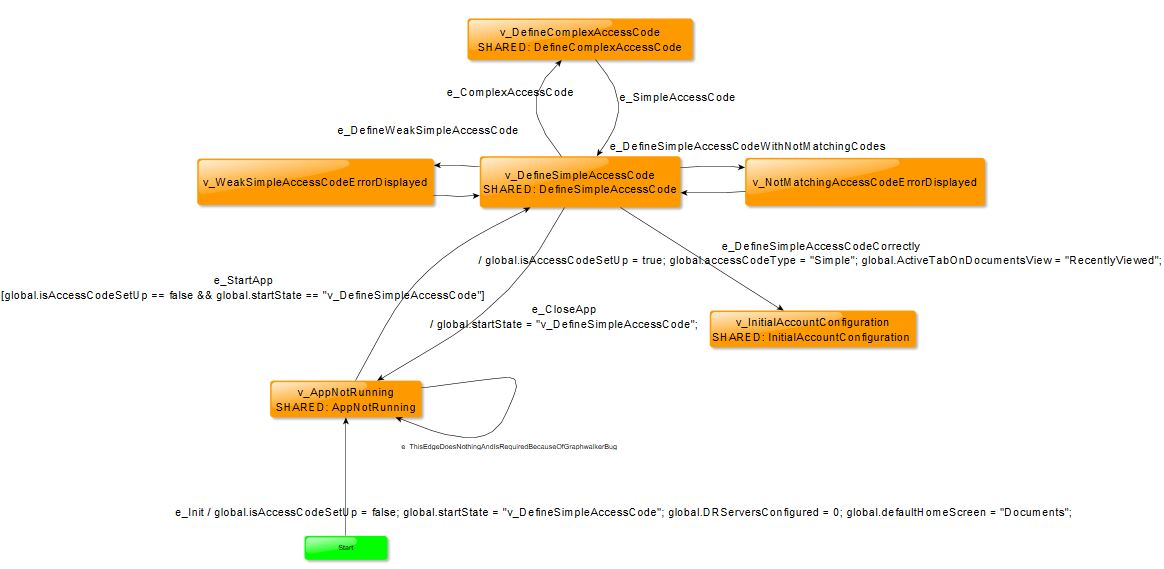
\includegraphics[width=1\textwidth]{figures/Authentication_model_screenshot}
					\caption{\label{Fig:Authentication_Model_Screenshot} Model for Define Simple Access Code feature}
\end{figure}

\subsection{Modeling of Navigation between tabs}
\par
After finishing authentication steps in \acrshort{bsc}, user is introduced to internal application functionality which consists of 5 tabs: documents tab, events tab, votes tab, datarooms tab and settings tab. One model is devoted for describing only navigation opportunities between these tabs. It contains all the possible transitions from one tab to another including closing the application from any tab. User is able to disable votes and events tabs from settings, so navigation model includes variables which are set in settings tab when enabling and disabling tabs and used in guards in navigation model. Model consists of 6 states and 25 transitions. It can be observed in figure \ref{Fig:Navigation_Model_Screenshot}.

\begin{figure} [htbp!]
	\centering
					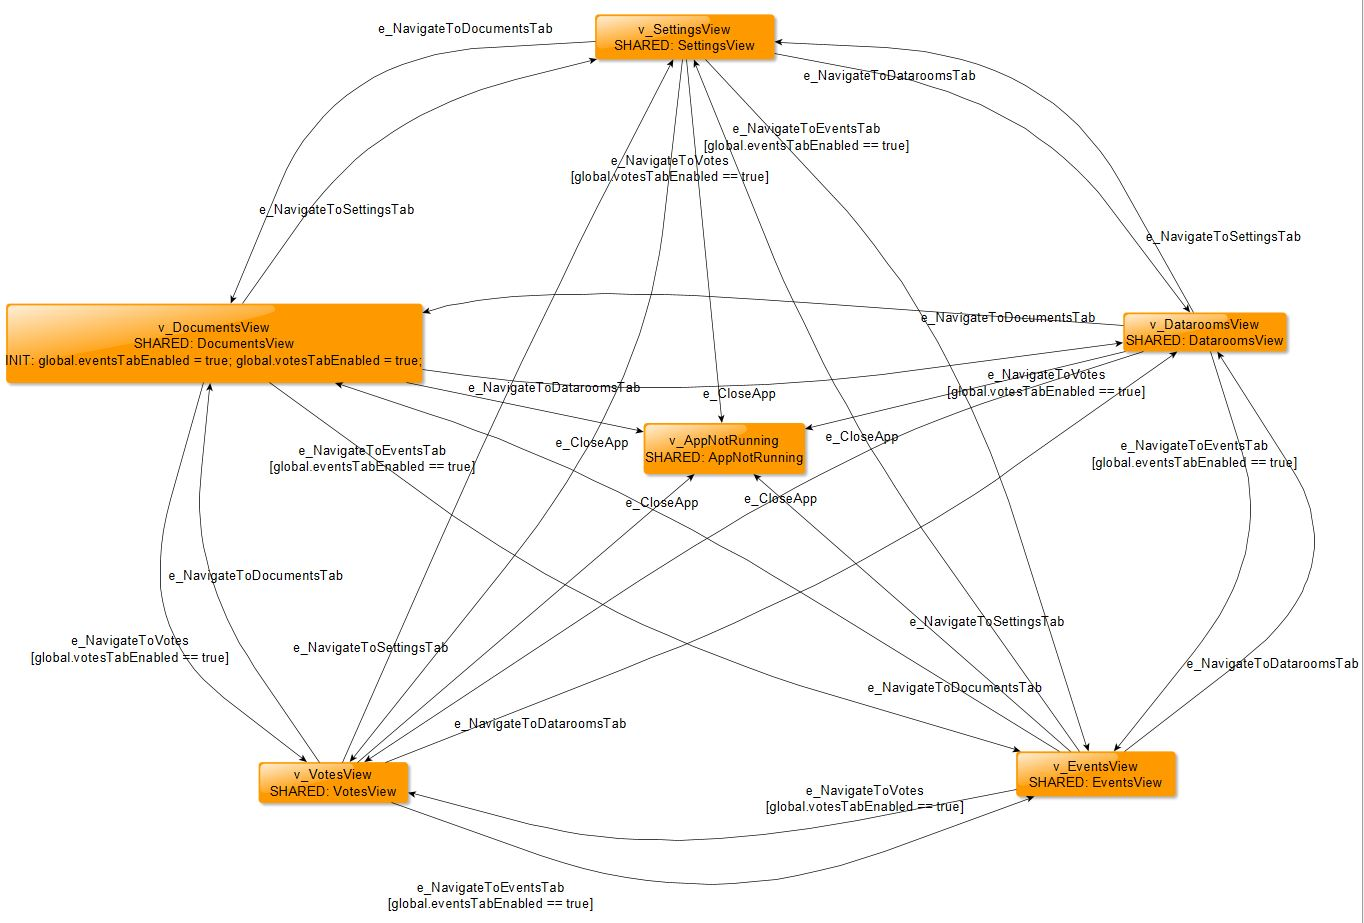
\includegraphics[width=0.92\textwidth]{figures/Navigation_model_screenshot}
					\caption{\label{Fig:Navigation_Model_Screenshot} Model for Navigation through Tabs}
\end{figure}

\subsection{Modeling of Documents Tab}
\par
Documents tab is most used tab in \acrshort{bsc} as it provides convenient representation of the documents in datarooms. It is split into 4 different filters for showing documents out of which 2 are permanently available. Recently viewed filter shows documents which were opened by user during the usage of \acrshort{bsc} sorted by accessing time in descending order. Recently changed filter displays documents which were recently added, edited or updated within the synchronized datarooms sorted by update date in descending order.

\par
Functionality of documents tab is split into 3 different models. Documents model is repsonsible for navigation between filters, while Recently Changed and Recently Viewed models are describe the functionality provided to user through these filters, such as accessing files different types of files content and context menus as well as navigation back to the respective filter. Recently viewed and recently changed models contain 7 states and 10 transitions each while documents model has 5 states and 20 transitions. Documents model can be observed in figure \ref{Fig:Documents_Model_Screenshot}. 

\begin{figure} [htbp!]
	\centering
					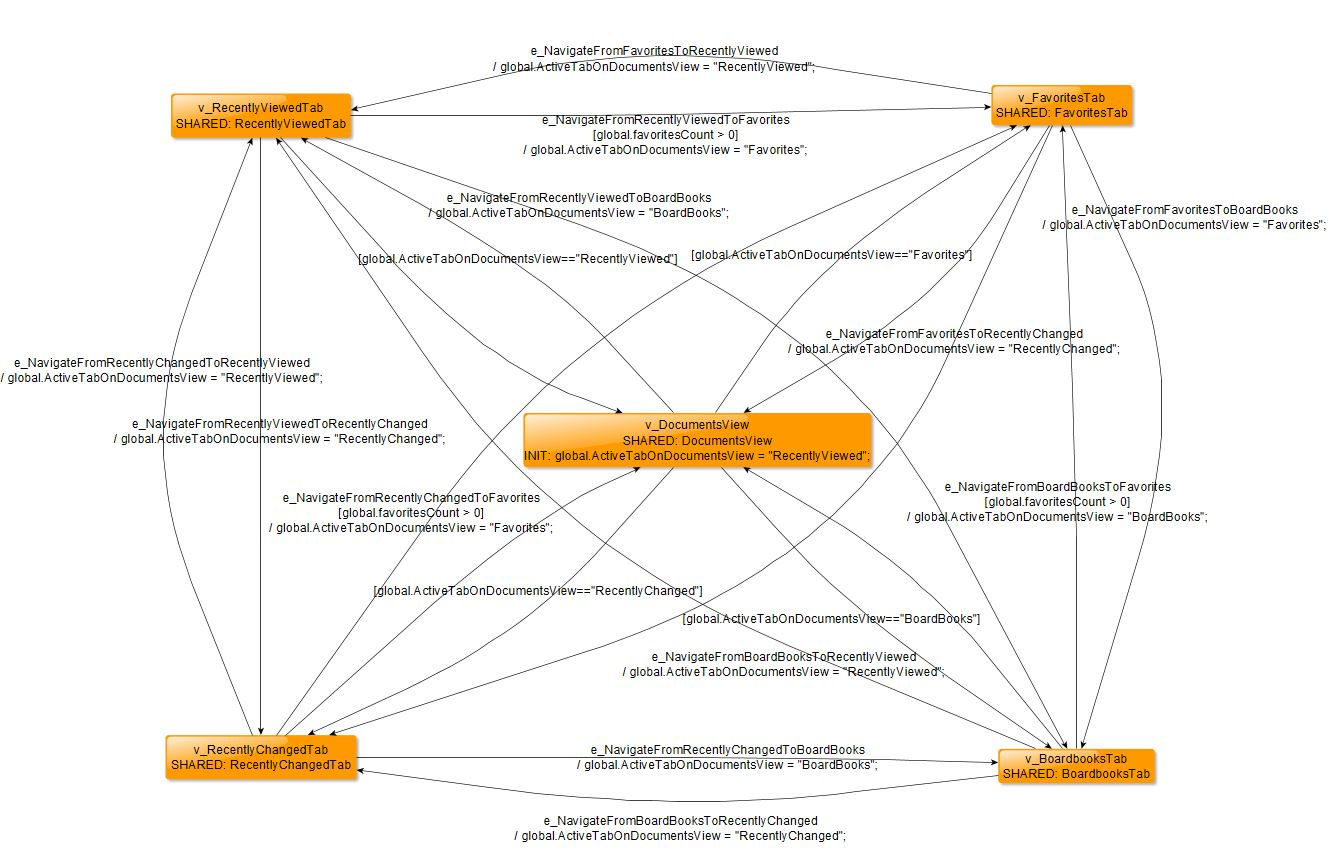
\includegraphics[width=0.92\textwidth]{figures/Documents_model_screenshot}
					\caption{\label{Fig:Documents_Model_Screenshot} Model for Documents Tab}
\end{figure}


\subsection{Modeling of Events Tab}
\par
Organizational events are one of the features of \acrshort{bdrs}. User can access created events of synchronized datarooms in \acrshort{bsc} on events tab. He/She has opportunity to filter events with different criteria such as, all events, past events, declined events, upcoming events and events for which his/her reply is pending. Displayed events can be sorted either by name or by due date. User has 3 options for replying event, accepting, declining and sending tentative response, after which the response is synchronized to \acrshort{bdrs}. User can observe other participants of the event as well as the attachments if available. Behavioral model of events tab consists of 16 states and 30 transitions and can be observed in figure \ref{Fig:Events_Model_Screenshot}.

\begin{figure} [htbp!]
	\centering
					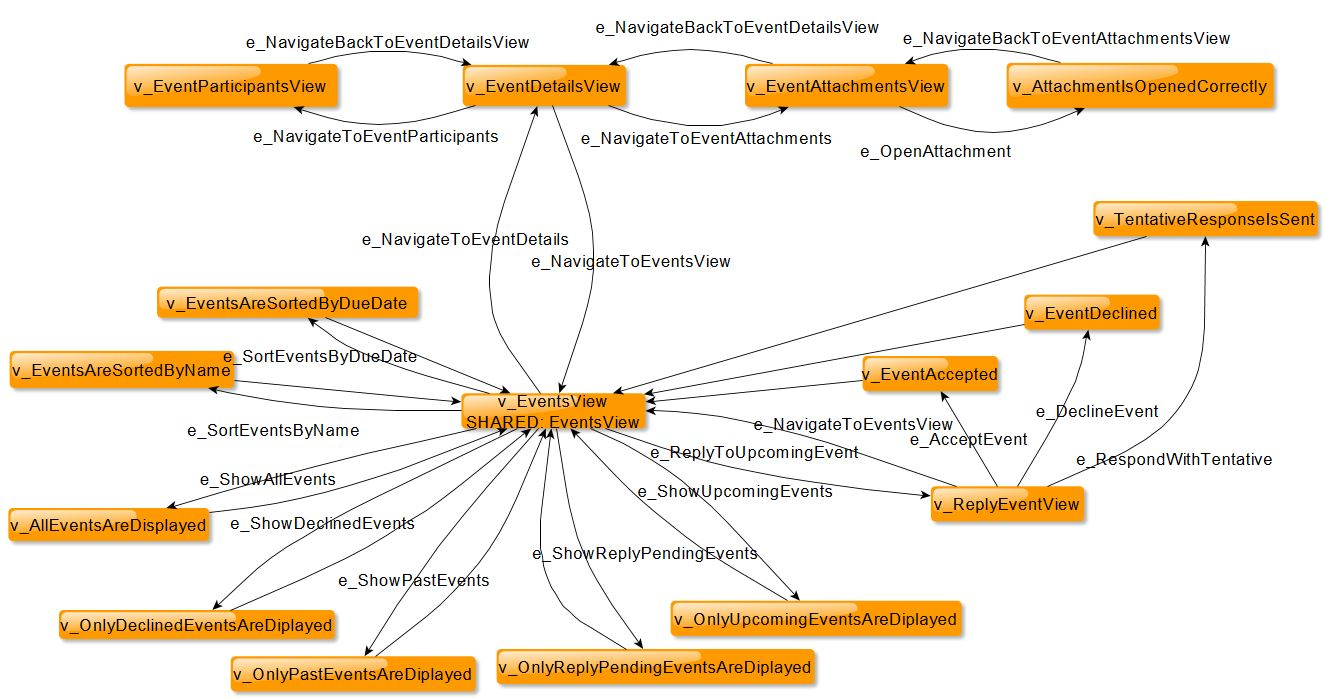
\includegraphics[width=1\textwidth]{figures/Events_model_screenshot}
					\caption{\label{Fig:Events_Model_Screenshot} Model for Events Tab}
\end{figure}

\subsection{Modeling of Votes Tab}
\par
\acrshort{bdrs} supports functionality of voting as well. User has ability to access votes of synchronized datarooms in \acrshort{bsc} on votes tab. Votes can be filtered with following criteria, all votes, in progress votes, closed votes and votes for which users choice is remaining. Similarly to events, votes also can be sorted either by name or by due date. 3 types of votes can be casted while voting, approve, decline and abstain. User can observe list of voters and attachments of the votes after expanding specific vote. Behavioral model of votes tab has 15 states and 30 transitions and can be observed in figure \ref{Fig:Votes_Model_Screenshot}.

\begin{figure} [htbp!]
	\centering
					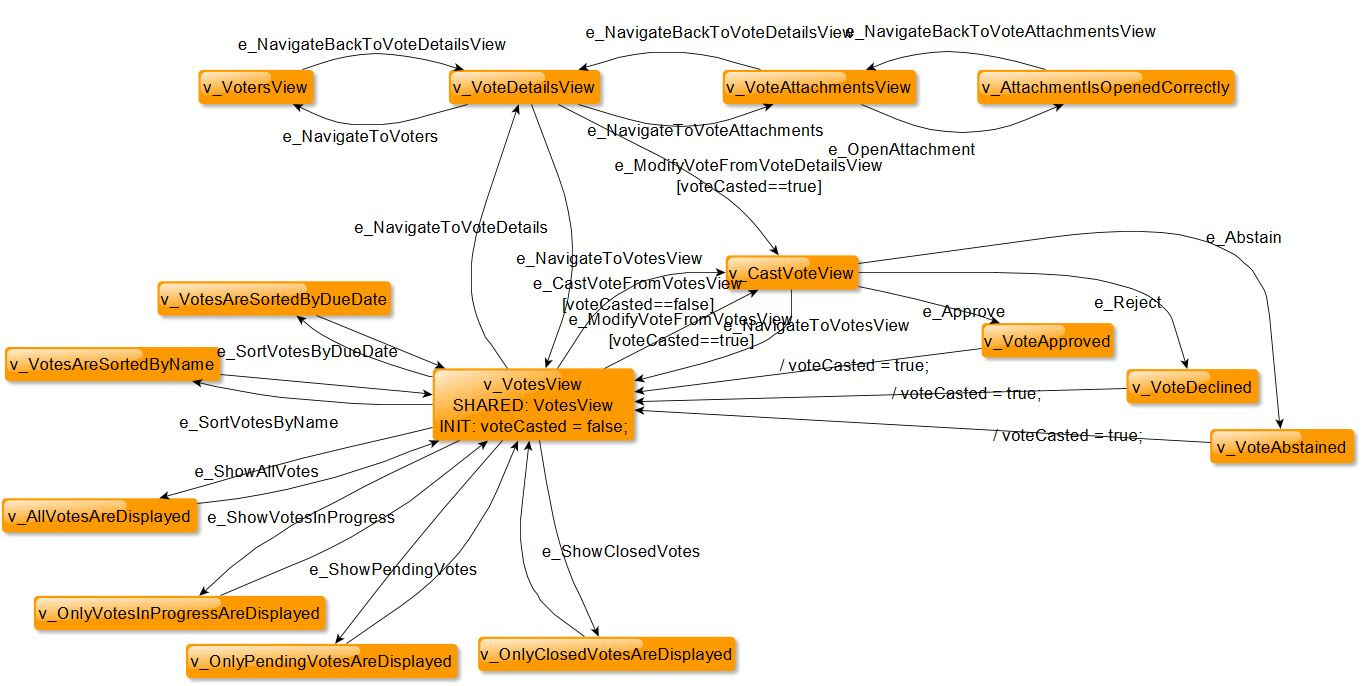
\includegraphics[width=1\textwidth]{figures/Votes_model_screenshot}
					\caption{\label{Fig:Votes_Model_Screenshot} Model for Votes Tab}
\end{figure}

\subsection{Modeling of Datarooms Tab}
\par
Datarooms tab is the part of \acrshort{bsc} where most of the application's functionality is embedded. User can access all datarooms to which he/she is invited on datarooms tab. He/She can navigate through datarooms and internal folder structure, create new folders at any level within the dataroom, upload new files from the device, download and open different versions of existing files locally either in original format or as generated protected PDF version. It is also possible to download complete content of the folder without downloading and opening each file. User can annotate protected PDF files, create different reviews of it and share them to different people invited to the dataroom where file is located. Last but not the least, user can send links of the files to email addresses of internal and external people based on the dataroom security policy.

\par
This huge set of functionality consisting of navigation, 4 different context menus, 2 different file viewers, as well as sharing and sending interfaces has been split into 11 different models. Datarooms model is orchestrating navigation to different modules of the tab. 4 models were dedicated to context menus, one to each. 3 models were created for original file viewer and PDF viewer. Separate models were created for sending links and sharing reviews which resulted in 2 more models and 1 model was created for viewer of all version of files. As context menus and PDF viewer has major share in functionality of datarooms tabs, they will be described separately in following subsections.

\par
Overall, all models together resulted in 143 states and 264 transitions. Datarooms model itself, which is responsible for navigation can be observed in figure \ref{Fig:Datarooms_Model_Screenshot}.

\begin{figure} [htbp!]
	\centering
					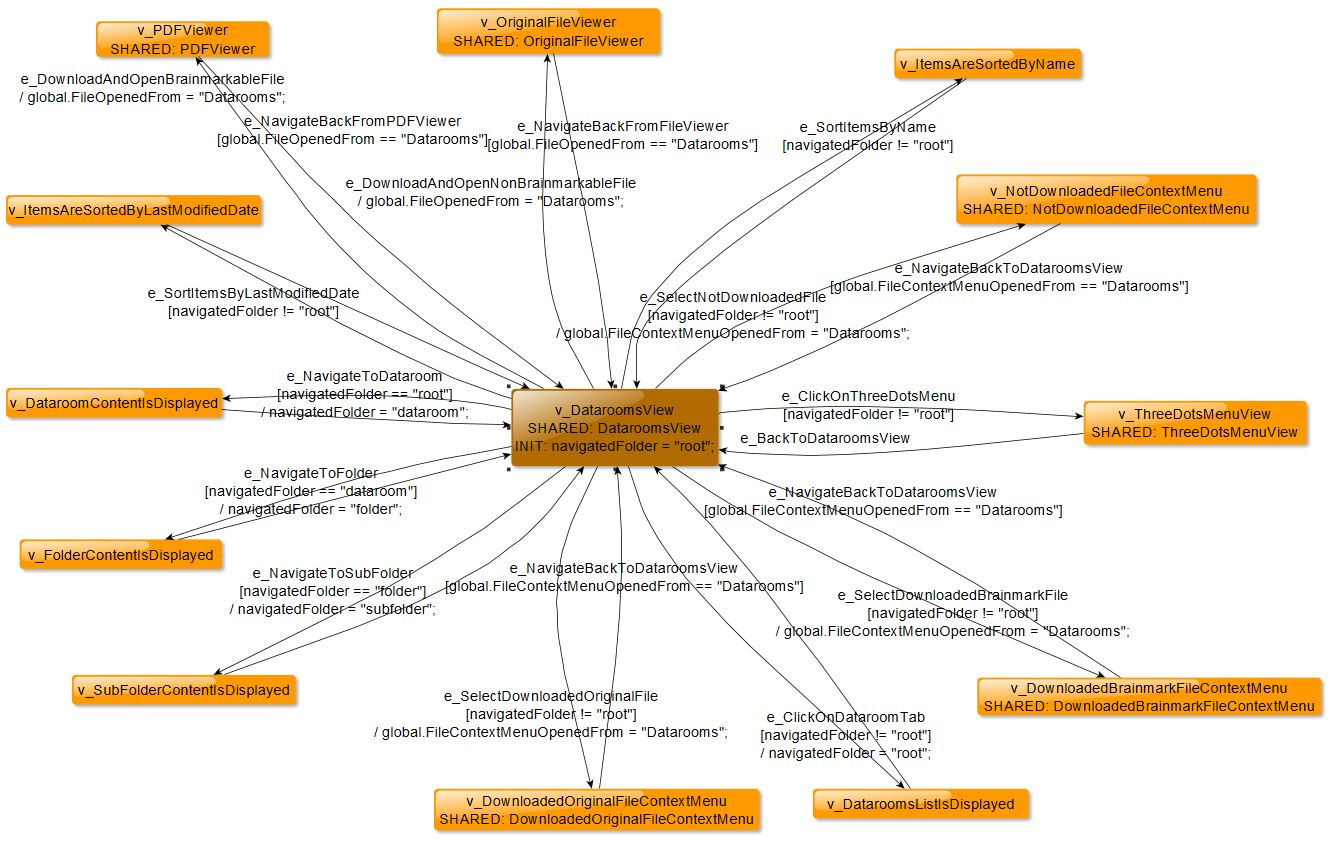
\includegraphics[width=1\textwidth]{figures/Datarooms_model_screenshot}
					\caption{\label{Fig:Datarooms_Model_Screenshot} Model for Datarooms Tab}
\end{figure}

\subsubsection{Modeling of Context Menus}
\par
Datarooms tab has 4 different context menus. Context menu for navigated dataroom or folder gives opportunity to create new folder, upload new file and download or delete locally all folders under navigated folder or dataroom. Model for this context menu has 11 states and 18 transitions and can be observed in figure below. Downloaded original file's context menu gives options for setting or unsetting file as favorite, viewing all versions of the file, showing votes to which selected file is attached, deleting file from device and sending file securely to internal or external email address. It has been modeled with 10 states and 21 transitions. Context menu of downloaded protected pdf file provides same options as downloaded original file's context menu and in addition to it user can share review of the file with users invited to the dataroom where file is located. Model has 11 states and 24 transitions. Context menu for not downloaded file gives same opportunities as one for downloaded file, but instead of option for deleting file locally, it gives option to download original file. Model for context menu of not downloaded file has 9 states and 18 transitions.

\begin{figure} [htbp!]
	\centering
					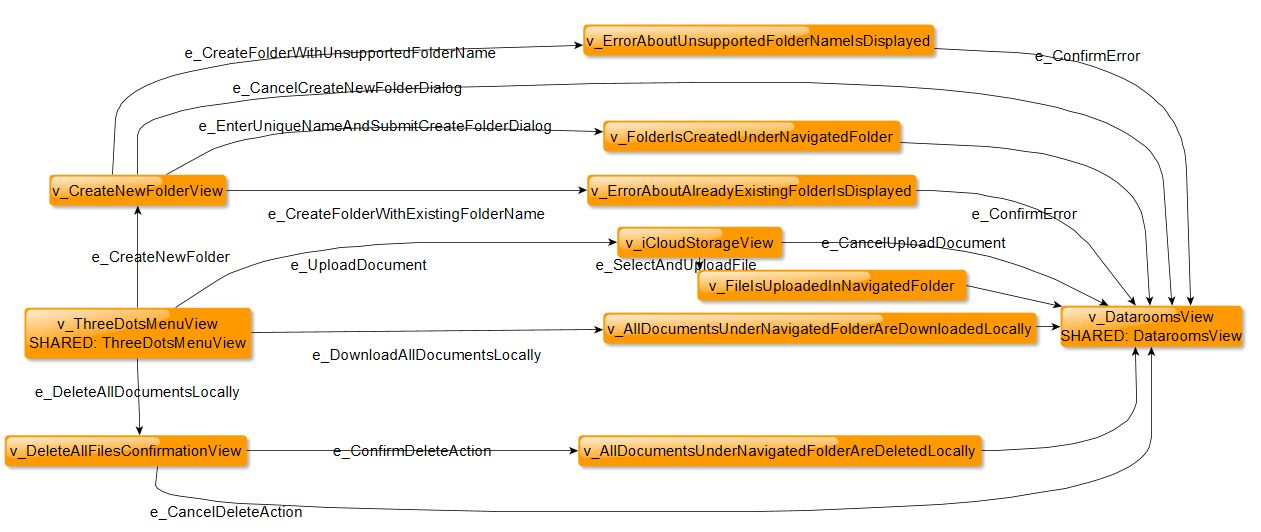
\includegraphics[width=1\textwidth]{figures/Context_Menu_model_screenshot}
					\caption{\label{Fig:Context_Menu_model_screenshot} Model for Dataroom Context Menu}
\end{figure}

\subsubsection{Modeling of PDF Viewer}
\par
PDF Viewer is one of the most important feature of \acrshort{bsc}. It allows user to open and read through generated protected PDF files, changing its views to fit page, fit width or fit height of document as well as changing layout of document as single page continuous or single page. User can search for different keywords within and navigate to found items through documents with search module. PDF document can be exported for printing directly from the PDF viewer as well as it can be exported to other applications on the device such as Notes. User is able to bookmark the pages within the document, and access them conveniently from thumbnails view. Different reviews can be accessed directly from PDF viewer's Reviews view and they can be directly shared to internal dataroom users. All this functionality is embedded in PDF Viewer Operations model. It contains 31 states and 58 transitions.

\par
The next huge set of functionality comes with possible annotations within PDF viewer. There are four types of annotations available: fineliner, pen, text and sticky notes. Eraser is also provided for deleting fineliner and pen annotation either completely or partially. User can create, edit or delete in case already created any type of annotation. Editing fineliner and pen annotations include changing color, changing thickness and changing opacity of the annotation. User can edit size and color of the text annotation as well as the content of the text itself. Sticky note annotations can be altered by changing text. Annotation related behaviour of PDF viewer related is Modeled in PDF Viewer Annotations model and consists of 26 states and 49 transitions.

\par
Unfortunately, due to huge size of models, none of them can be displayed visually in this thesis as reader will not be able to read labels of states and transitions.

\subsection{Modeling of Settings Tab}
\par
Settings tab allows user to configure internal settings of application accroding to his/her needs. 
\par
Through application view settings user can set the default starting tab of application after entering access code, can hide and show events and votes tab and if auto-indexing is enabled and configured within dataroom user can show and hide these indexes. 
\par
Access code settings make user eligible for changing defined access code.
\par
Security settings allow user to change password for already connected accounts, reset secondary authentication, logout of all the configured dataroom server accounts, set the period for auto lock functionality, allow or restrict user for copying texts through \acrshort{bsc} and pasting them in some other applications. Also user can restrict or allow the device to include data from \acrshort{bsc} into iOS backup. 
\par
Download settings can be used in case user wants to activate, deactivate or set default download period of the items in synchronized datarooms. He/She can observe ongoing downloads in download settings. Also, user can restrict app to download items only in case if device is connected to Wi-Fi or another option can be set which allows download even in case when mobile network is used. 
\par
Through deletion settings user can delete all local content of the application, can set the default time period after which local documents will be automatically deleted and also can reset application completely which will delete all local content, will log out from all logged in accounts and will reset the defined access code.
\par
Servers and Datarooms settings allow user to add or remove dataroom servers as well as synchronize or remove datarooms from added dataroom servers to which he/she is invited.
\par
Support view allows user to access and read through data such as user guide, setup guide, legal and data protection notices. User is also able to send log files or contact support in Brainloop via support tab and can access customer service portal.
\par
Settings functionality is split up into 11 models. One main model is responsible for navigation between listed settings. It can be observed in figure below. Each 7 settings of \acrshort{bsc} have dedicated models. 3 more models are created for security settings and servers and datarooms settings as they were complex and required splitting.

\begin{figure} [htbp!]
	\centering
					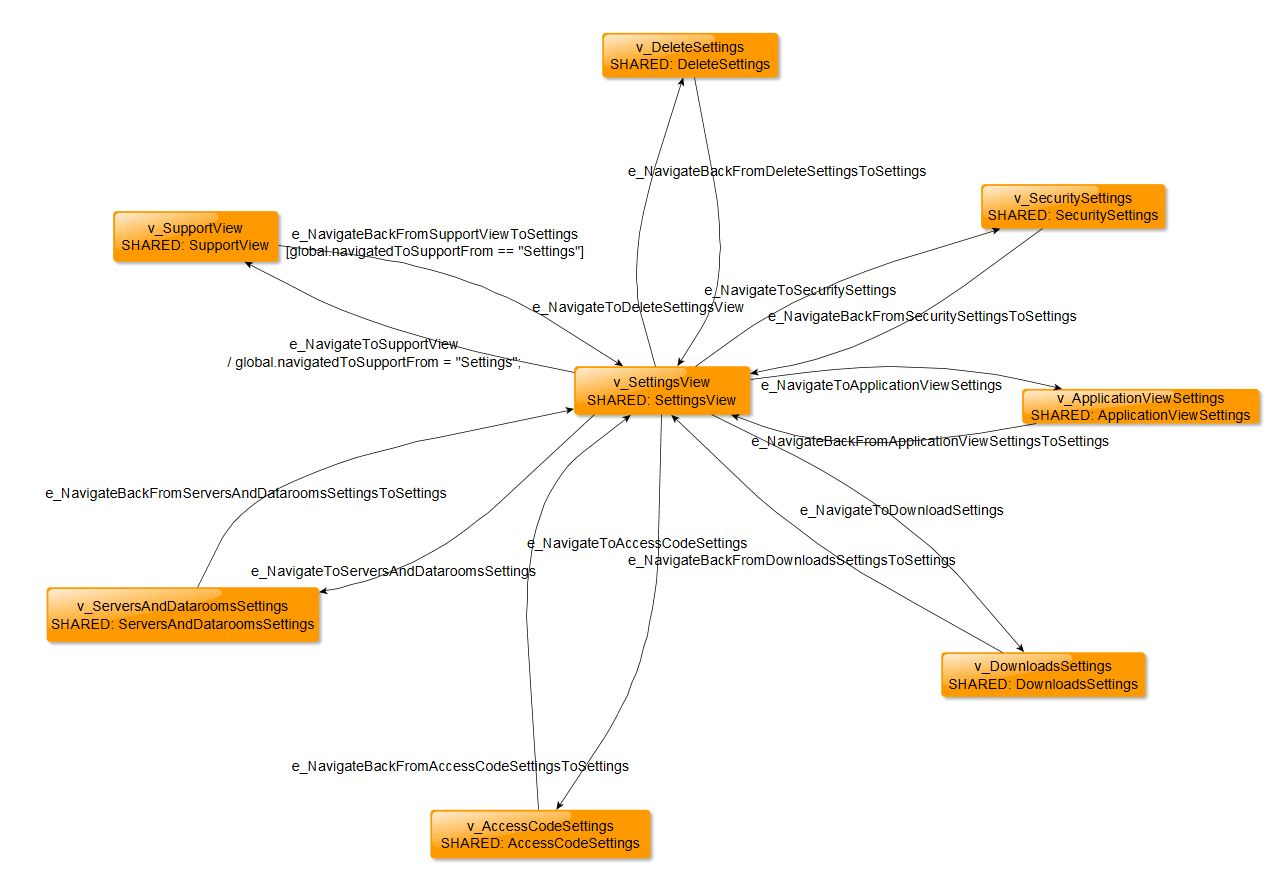
\includegraphics[width=1\textwidth]{figures/Settings_model_screenshot}
					\caption{\label{Fig:Settings_model_screenshot} Model for Settings Tab}
\end{figure}

\section{Layers}
\par
Created models are structured in layered manner. Accessing the specific functionality requires passing through all the layers between Base layer and the layer where functionality is described. The best practice would be if none of models depend on any model below the layer where it resides. But, unfortunately, in some cases that can not be achieved. For example, application view settings decide on which tab will user land after entering the access code and landing on specific tab is decided in enter access code model which resides in base layer. There are very few exceptions like this in models, but they were worth mentioning. Figure \ref{Fig:Layers} describes detailed structure of layers of our models.

\begin{figure} [htbp!]
	\centering
					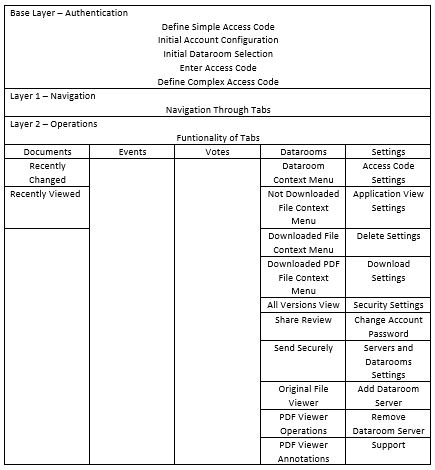
\includegraphics[width=0.8\textwidth]{figures/Layers}
					\caption{\label{Fig:Layers} Layered Structure of Models}
\end{figure}

\section{Sum Up}
\par
Overall, 33 models were created, with total 312 states and 566 transitions describing behavior of \acrshort{bsc}. More detailed representation of states and transitions can be observed in table \ref{tab:Behavioral_models}.


\begin{table}[]
    \centering
    \begin{tabular}{|l|l|l|}
        \hline
        \textbf{Model Name} & \textbf{States} & \textbf{Transitions} \\
        \hline
        Datarooms & 13 & 25 \\
        \hline
        Dataroom Context Menu & 11 & 18 \\
        \hline
        Define Complex Access Code & 5 & 7 \\
        \hline
        Define Simple Access Code & 7 & 10 \\
        \hline
        Documents & 5 & 20 \\
        \hline
        Recently Changed & 7 & 10 \\
        \hline
        Recently Viewed & 7 & 10 \\
        \hline
        Enter Access Code & 8 & 11 \\
        \hline
        Events & 16 & 30 \\
        \hline
        All Version View & 3 & 4 \\
        \hline
        File Context Menu - Downloaded & 10 & 21 \\
        \hline
        File Context Menu - Not Downloaded & 9 & 18 \\
        \hline
        File Context Menu - Downloaded PDF & 11 & 24 \\
        \hline
        Share Review & 12 & 19 \\
        \hline
        Send Securely & 13 & 23 \\
        \hline
        Initial Account Configuration & 6 & 9 \\
        \hline
        Initial Dataroom Selection & 9 & 13 \\
        \hline
        Navigation Through Tabs & 6 & 25 \\
        \hline
        Original File Viewer & 4 & 6 \\
        \hline
        PDF Viewer Operations & 31 & 58 \\
        \hline
        PDF Viewer Annotations & 26 & 49 \\
        \hline
        Settings & 8 & 14 \\
        \hline
        Access Code Settings & 2 & 5 \\
        \hline
        Application View Settings & 9 & 16 \\
        \hline
        Delete Settings & 4 & 5 \\
        \hline
        Download Settings & 9 & 16 \\
        \hline
        Security Settings & 10 & 18 \\
        \hline
        Change Account Password & 5 & 6 \\
        \hline
        Servers and Datarooms Settings & 14 & 22 \\
        \hline
        Add Dataroom Server & 5 & 6 \\
        \hline
        Remove Dataroom Server & 4 & 4 \\
        \hline
        Support & 8 & 14 \\
        \hline
        Votes & 15 & 30 \\
        \hline
        \textbf{Total} & \textbf{312} & \textbf{566} \\
        \hline
    \end{tabular}
    \caption{Behavioral Models of \acrshort{bsc}}
    \label{tab:Behavioral_models}
\end{table}














